\chapter{Comparaisons d'algorithmes}
\label{chap:resultats_comparaisons}


\section{Les méthodes pratiques} 
\label{sec:methodes_pratiques}
Nous cherchons maintenant à déterminer les performances et les qualités des différents algorithmes de proteus.
Pour évaluer les différents algorithmes de proteus, comme pour leur établir un paramétrage, nous effectuons des séries de tests. 
Grâce à l'algorithme de type toulbar2 il est possible d'obtenir la séquence/conformation qui possède la plus haute énergie de dépliement. Cela constitue une information important qui va nous servir d'élément de comparaison.Le facteur temps est également un élément déterminant. Il est dans certain cas limitant, nous ne savons pas à l'avance quand toulbar2 termine. Et il apparaît d'emblée illusoire d'espérer voir ce programme converger dans toutes les situations intéressantes dans un temps raisonnable.D'autres métriques qui caractérisent les séquences d'acides aminés de meilleurs énergies obtenues seront également utilisées pour les évaluations et pour les paramétrages.   

Dans la suite, on appelle «position active», une position pour laquelle, tous les types d'acides et tous les rotamères de chaque type d'acide aminé sont autorisés, au court de la recherche de proteus. On désigne «séquence/conformation» une séquence d'acides aminés munie à chaque position d'un rotamère (le backbone étant de toute façon fixé).Tandis ce que le terme simple «séquence»  sans plus de précision désigne une séquence d'acides aminés.


\subsection{les protéines}
 
Les tests sont effectués sur neuf protéines choisies pour avoir des longueurs de backbone variées, plusieurs domaines représentés, mais aussi plusieurs structures pour chaque famille présente. Ainsi l'ensemble se décompose en deux protéines SH3 de 56 et 57 résidus, de trois protéines PDZ de longueur comprise entre 82 et 97 résidus  et enfin de trois protéines SH2 longues de 105 ou 109 résidus.L'ensemble a une moyenne, arrondie à l'unité inférieure, de quatre-vingt-neuf positions, voir les détails en table~\ref{tab:protéines}. 
  

    \begin{table}[!htbp]
      \centering

      \begin{tabular}{cccc}

        \toprule
        Code PDB & résidus & nombre de positions & domaine\\
        \cmidrule{1-4}
        1ABO & 	64-119	 & 	56	 & SH3 \\
        1CKA & 	134-190	 & 	57	 & SH3 \\
        1R6J & 	192-273	 & 	82	 & PDZ \\
        1G9O & 	9-99	 & 	91	 & PDZ \\
        2BYG & 	186-282	 & 	97	 & PDZ \\
        1BM2 & 	55-152	 & 	98	 & SH2 \\
        1O4C & 	1-105	 & 	105	 & SH2 \\
        1M61 & 	4-112	 & 	109	 & SH2 \\
        1A81 & 	9-117	 & 	109	 & SH2 \\
        \bottomrule

      \end{tabular}      
      \caption{Les protéines}
\label{tab:protéines}      
    \end{table}




\paragraph{Alignements Blast croisés}


    \begin{table}[!htbp]
      \centering

      \begin{tabular}{ccc}

        \toprule
     Protein & 1ABO  & 1CKA  \\
        \cmidrule{1-3}
        1ABO & 100 (6e-42) &  26 (1e-07) \\     
        1CKA &  26 (1e-07) & 100 (2e-41) \\
        \bottomrule


      \end{tabular}      
      \caption{Pourcentage d'identité et e-value des alignements Blast native vs native pour nos protéine SH3.}
\label{tab:Xblast_SH3}      
    \end{table}

    \begin{table}[!htbp]
      \centering

      \begin{tabular}{cccc}

        \toprule
     Protein & 1R6J & 1G9O & 2BYG  \\
        \cmidrule{1-4}
        1R6J & 100(1e-59) & 25 (3e-07) & no          \\ 
        1G9O & 25 (3e-07) & 100(2e-66) & 35 (2e-11)  \\
        2BYG & no         & 35 (2e-11) & 100(7e-71)  \\
        \bottomrule


      \end{tabular}      
      \caption{Pourcentage d'identité et e-value des alignements Blast native vs native pour nos protéine PDZ (no= pas de touche avec une e-value inférieure à 10).}
\label{tab:Xblast_PDZ}      
    \end{table}


    \begin{table}[!htbp]
      \centering

      \begin{tabular}{ccccc}

        \toprule
     Protein & 1BM2  & 1O4C  & 1M61 & 1A81 \\
        \cmidrule{1-5}
        1BM2 & 100 (7e-74) &  36 (2e-16) &  38(6e-10) &  35 (1e-13) \\
        1O4C & 36  (2e-16) &  100(2e-79) &  27(3e-10) &  33 (2e-12) \\
        1M61 & 38  (6e-10) &  27 (3e-10) & 100(6e-81) &  57 (2e-47) \\
        1A81 & 35  (1e-13) &  33 (2e-12) &  57(2e-47) &  100(5e-83)  \\
        \bottomrule
      \end{tabular}
      \caption{Pourcentage d'identité et e-value des alignements Blast native vs native pour nos protéine SH2.}      
\label{tab:Xblast_SH2}      
    \end{table}


    \begin{figure}[h]
      \centering
      \begin{tabular}{cc}
        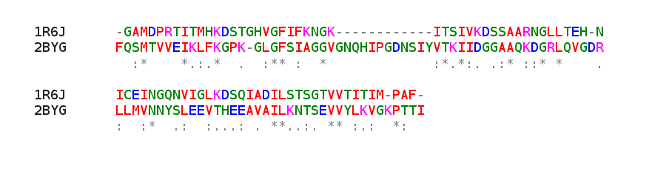
\includegraphics[width=18cm]{align_clustalo_1R6Jvs2BYG.png} 
      \end{tabular}
      
      \caption{alignement de 1R6J et 2BYG obtenu avec Clustal Omega version 1.2.1}
\label{graph:all_result}
    \end{figure}

\clearpage

\subsection{Description des tests}
\label{sec:description_tests}
Les tests sont répartis en deux ensembles:
\begin{enumerate}
\item un ensemble de tests où toutes les positions de la séquence sont actives (cela correspond aux situations de design complet de protéines) 
\item un ensemble de tests où le nombre de positions actives est gardé sous contrôle de façon à maîtriser la taille de l'espace d'exploration
\end{enumerate}


\paragraph{Ensemble «Tout actif»}
\label{methode_TTactif}
Pour le premier ensemble de tests,la totalité de la matrice d'énergie est exploitée et pour chaque position l'espace d'exploration correspond à l'espace d'état déclaré dans le fichier ".bb".C'est-à-dire que tous les types de résidu et tous les rotamères sont possibles à chaque position.
Comme l'espace des séquences/conformations à explorer est gigantesque, nous ne faisons pas de tentatives de recherche du GMEC  par méthode exacte. 

Nous effectuons des recherches avec les algorithmes suivants:

\begin{itemize}
\item heuristique, noté H par la suite;
\item Monte-Carlo, noté MC;
\item «Replica Exchange», noté RE);
\end{itemize}


\paragraph{L'ensemble «nombre d'actifs limité»}

L'ensemble «Nombre d'actifs limité» est composé de six groupes de tests avec un nombre de positions actives fixe définit de la façon suivante:  


\begin{enumerate}
\item aucune position active
\item une position active 
\item cinq positions 
\item dix  positions 
\item vingt positions 
\item trente positions 
\end{enumerate}

Lorsqu'une position n'est pas active,l'acide aminé de la position est fixé en utilisant l'acide aminé de la séquence native. La chaîne latérale est, elle, laissée libre. Il n'y a donc jamais dans nos tests de position où l'état est complètement fixé.

Le groupe «aucune position active» n'est constitué que d'un test par algorithme pour chaque protéine. Il y a donc neuf tests par algorithme.
Ce sont les tests pendant lesquels la séquence d'acides aminés est fixe et correspond à la séquence native de la protéine.

Pour les tests avec une seule position active, comme des temps de calcul le permettent, nous décidons d'être exhaustifs:
Toutes les positions sont testées, il y a alors huit cent quatre tests par algorithme.
Pour tous les autres groupes de tests (cinq,dix,vingt et trente positions actives), cinq tests sont effectués par protéine, c'est-à-dire quarante-cinq tests par algorithme.

\paragraph{le choix des positions actives}
\label{para:choix_posi}
Pour définir complètement les tests, il reste maintenant à décrire le choix des positions actives pour les groupes de numéro trois jusqu'à six.
Il y a peu d'intérêt à tester des situations avec des positions actives sans interaction entre-elles.
En effet, s'il existe une position active P dont chaque résidu est sans interaction avec tous les résidus possibles des autres positions actives, déterminer le meilleur état pour P est proche du test du groupe 2 avec P comme position active. Toutefois, cela n'est pas exactement la même question, parce que les positions actives différentes de P peuvent influencer la position de la chaîne latérale de positions inactives qui à leur tour peuvent influencer l'état de P.
Ainsi, le choix des positions actives ne se fait non pas par tirage aléatoire, car le risque d'obtenir des positions avec peu d'interactions est trop grand. Il se fait sous contrainte d'interaction.

\paragraph{positions en interactions}
Pour cela, nous utilisons la notion de voisinage de proteus. Elle se définit de la façon suivante:  
Deux positions P et Q sont en interactions s'il existe un rotamère $r_P$ de P et un rotamère $r_Q$ de Q tels que:
\begin{displaymath}
 | E(r_P,r_Q) | > S_{Vois}
\end{displaymath} 
avec $S_{Vois}$ un seuil donné par l'utilisateur à la configuration de proteus (voir chap. ?? pour les détails).

Alors on appelle «n-uplet en interaction» la donnée de n positions avec $n \in \{5,10,20,30\}$ et d'un seuil  $S_{Vois}$  tels que pour toute paire de positions (P,Q) du n-uplet, P et Q sont en interactions.
\paragraph{choix des  positions actives}
Pour définir les positions actives,nous exécutons proteus en mode verbeux, sans effectuer d'optimisation.Pour cela,
il existe plusieurs façons de procéder, ici nous utilisons le mode Monte-Carlo avec une trajectoire de zéro pas. Ces exécutions produisent en sortie standard la liste des voisins pour chaque position au seuil donnée en paramètre.
Pour chacune des neuf protéines, nous exécutons proteus avec $S_{Vois}$ égal à dix, cinq et un à tour de rôle; trois listes de voisins sont obtenues. 
Ensuite,un script dédié recherche dans ces listes, les n-uplets en interaction, en partant de la liste de voisins au sens le plus fort, c'est-à-dire dix, vers celle  au sens le plus faible ($0.1$).La recherche s'arrête lorsque cinq n-uplets au moins sont trouvés.

Nous obtenons quarante-cinq n-uplets pour le groupe à cinq (respectivement dix, vingt et trente ) positions actives pour un seuil $S_{Vois}$ égal à dix (respectivement dix, un et un). Les positions actives de tous les tests sont en annexe~\ref{chap:annexe1 }).Pour chaque n-uplet, un fichier de configuration de proteus est créé dans lequel la balise <Space\_Constraints> fixe les positions inactives en utilisant le type d'acide aminé présent dans la séquence native. 


\subsection{Définition de protocole comparable}
\label{sec:proto_compa}
Nous voulons comparer les algorithmes très différents. Un algorithme peut garantir l'obtention du minimum global en énergie (GMEC) si l'exécution se termine, mais ne garantit pas qu'elle se termine. Un autre permet un contrôle très fin du temps d'exécution sans garantie du GMEC, et d'autres enfin ont des objectifs plus large que la seule obtention du GMEC.
Mais le GMEC reste le meilleur point de commun. Nous allons donc y concentrer une part importante des comparaisons.

Nous devons noter également que l'obtention du GMEC est théorique, en pratique nous n'avons pas de preuve que le code de l'algorithme exact que nous utilisons n'a pas de bogue. Cependant,nous mettons de côté cette éventualité et dans toute la suite GMEC désigne aussi bien le minimum global en énergie que le résultat de toulbar2 lorsqu'il se termine.  
Le Monte-Carlo et le «Replica exchange» possèdent de nombreux paramètres de configuration, ce qui rend l'ensemble des protocoles possibles très grand. Se pose alors la question de l'optimisation du protocole. L'objectif fixé ici,n'est pas la recherche d'un protocole optimal pour chacun des tests, mais d'évaluer, avec les tests, un protocole optimisé par algorithme.
Nous allons alors dans un premier temps, recherche les meilleurs paramétrages pour le Monte-Carlo et le «Replica Exchange» sur l'ensemble de tests «tout actif».
Puis, sur la base des résultats obtenus, les protocoles seront fixés pour effectuer les comparaisons sur l'ensemble  «tout actif» et celui à «nombre d'actifs limité».
Le programme toulbar2 possède aussi de nombreuses options. Deux paramétrages différents seront utilisés.

Pour rendre les protocoles comparables, le temps d'exécution maximum est fixé à vingt-quatre heures pour tous les exécutions.
Toulbar2 donne sa meilleure séquence/conformation en dernier, il n'y a donc pas post-traitement nécessaire.
C'est également le cas pour le Monte-Carlo à condition de configurer l'impression de la trajectoire avec la balise $Print\_Threshold=0$. dans le fichier de configuration.
Pour le "Replica Exchange" et l'heuristique, un tri des séquences selon l'énergie est nécessaire. Mais il n'y a pas beaucoup de séquences: 
\begin{enumerate}
\item L' Heuristique fournit une séquence/conformation à chaque cycle.
\item Le "Replica Exchange avec $Print\_Threshold=0$ produit autant de fichiers de séquences/rotamères que de marcheurs.Chacun ne contenant pas plus de quelques dizaines de séquences/rotamères. 
 \end{enumerate}

Nous pouvons donc négliger la durée du tri dans le temps total d'exécution.    

\paragraph{Protocole heuristique}

Pour l'algorithme heuristique, il n'y a dans notre situation qu'un seul paramètre à renseigner: le nombre de cycles à effectuer. Quelques essais préliminaires sur la plus grosse protéine (Table~\ref{tab:protéines}) avec toute les positions actives, montre que la version utilisée de proteus peut effectuer jusqu'à environ 110000 cycles sur nos machines de calculs en l'espace de vingt-quatre heures. Ainsi, le protocole H est défini comme le protocole qui utilise le mode heuristique de proteus et qui effectue cent dix mille cycles. Sont également définis les variantes H-, H+ et H++ comme des protocoles plus courts ou plus longs à facteur entier près (Table~\ref{tab:protoH}). Par ailleurs, certaines comparaisons de l'heuristique avec le Monte-Carlo ont été faites avec une version précédente du programme proteus.Ce protocole sera noté h. Il diffère aussi de H par le fait que l'option d'optimisation du compilateur Intel utilisé est -O2 contre -O3 pour H.    


    \begin{table}[!htbp]
      \centering

      \begin{tabular}{lr}

        \toprule
        Nom & nombre de cycles \\
        \cmidrule{1-2}
        H   & 110000 \\  
        H-  & 1100   \\  
        H+  & 330000 \\  
        H++ & 990000 \\  
        h   & 100000 \\  
        \bottomrule

      \end{tabular}      
      \caption{Les protocoles heuristiques}
\label{tab:protoH}      
    \end{table}

   \paragraph{Protocoles Monte-Carlo}
\label{para:MC}
On distingue deux ensembles de protocoles Monte-Carlo.Dans le premier, les noms  sont de la forme "mc*". Il rassemble les protocoles utilisés pour le paramétrage du Monte-Carlo.Le second est constitué des protocoles utilisés lors des comparaisons.     

Les éléments à paramétrer pour l'algorithme Monte-Carlo sont les suivants:

\begin{enumerate}
\item la température
\item le nombre de pas (avec le nombre de trajectoires et la longueur de trajectoire )
\item Le seuil de voisinage
\item Les probabilités de changements de la séquence/conformation
\end{enumerate}

Ce qui représente un ensemble de protocoles trop grand pour une approche exhaustive. Pour l'essentiel, nous allons faire varier les paramètres un par un, en prenant comme point de départ un protocole qui rend le comportement de marcheur Monte-Carlo «proche» de l'heuristique.

La température est le paramètre principal du Monte-Carlo, c'est elle qui contrôle le taux d'acceptation du critère de Metropolis.Alors,la première étape de cette optimisation va consister à faire varier la température , entre 0.001 et 0.5 , en conservant les autres paramètres fixés (protocoles de mc0 à mc5).Le nombre de pas total effectué est le produit de deux paramètres, le nombre de trajectoires et la longueur de trajectoire. Les protocoles mc1b et mc2b testent l'effet d'une augmentation du nombre de pas. Tandis que mc2c et mc2d testent l'effet de la variation du nombre de trajectoires par rapport à la longueur.
Le protocole mc2e s'intéresse aux probabilités de changement de la trajectoire. Il y a cinq balises dans proteus qui contrôle ces changements:

\begin{description}
\item[<Prot>] donne la probabilité de modifications de  rotamère à une position.
\item[<Prot\_Prot>] donne la probabilité de modifications de  rotamère à deux positions.
\item[<Mut>] donne la probabilité de modifications de type de résidu à une position.
\item[<Mut\_Prot>] donne la probabilité de modifications de  rotamères à deux positions.
\item[<Mut\_Mut>] donne la probabilité de modifications de type de résidu à deux positions.
\end{description}

La table~\ref{tab:protoMC} donne les probabilités utilisées par ces cinq paramètres dans l'ordre de la liste précédente. 

Enfin, mc4b se distingue des autres par un seuil de voisinage plus grand ((Table~\ref{tab:protoMC})).

\paragraph{Seconde version de proteus}
Pour la partie comparaison avec les autres algorithmes, quatre protocoles sont utilisés. Les protocoles MCa et MCb s'inspirent fortement de mc2d et mc2e , en étant adapté à la contrainte du temps de calcul de la comparaison et en utilisant la nouvelle version de proteus (les lettres capitales dans le nom des protocoles signifient l'utilisation de la dernière version de proteus). MCa- est une variante de MCa avec une trajectoire six fois plus courte.Enfin, MC0 s'inspire de mc0 dans le sens où la température est suffisamment froide pour que nous puissions considérer qu'il n'y a pas de baisse de l'énergie au cours d'une trajectoire.
  

    \begin{table}[!htbp]
      \centering

      \begin{tabular}{llrrcc}

        \toprule
        Nom & Temp & Long. de trajectoire(mega) & Nb de trajectoires  & Voisin & Proba \\
        \cmidrule{1-6}
        mc0   & 0.001 &  3  &  1000  & 10 & 0; 1; 0.1; 0 ;0 \\      
        mc1   & 0.1   &  3  &  1000  & 10 & 0; 1; 0.1; 0 ;0 \\  
        mc2   & 0.2   &  3  &  1000  & 10 & 0; 1; 0.1; 0 ;0 \\ 
        mc3   & 0.3   &  3  &  1000  & 10 & 0; 1; 0.1; 0 ;0 \\               
        mc4   & 0.5   &  3  &  1000  & 10 & 0; 1; 0.1; 0 ;0 \\  
        mc5   & 0.7   &  3  &  1000  & 10 & 0; 1; 0.1; 0 ;0 \\  
        mc1b  & 0.1   &  6  &  1000  & 10 & 1; 1;   1; 1 ;0 \\  
        mc2b  & 0.2   &  6  &  1000  & 10 & 0; 1; 0.1; 0 ;0 \\      
        mc2c  & 0.2   &  3  & 10000  & 10 & 0; 1; 0.1; 0 ;0 \\   
        mc2d  & 0.2   &  3000  &  1 & 10  & 0; 1; 0.1; 0 ;0 \\ 
        mc2e  & 0.2   &  3  &  1000  & 10 & 1; 0; 0.1; 0 ;0 \\     
        mc4b  & 0.5   & 10  &   100  & 10 & 0; 1;   0; 1 ;0 \\
        \cmidrule{1-6}
        MC0   & 0.01  &  1000  &  1  & 10 & 1; 0; 0.1; 0 ;0 \\            
        MCa   & 0.2   &  6000  &  1  & 10 & 1; 0; 0.1; 0 ;0 \\   
        MCa-  & 0.2   &  1000  &  1  & 10 & 1; 0; 0.1; 0 ;0 \\   
        MCb   & 0.2   &  6000  &  1  & 10 & 0; 1; 0.1; 0 ;0 \\      

        \bottomrule   
        
      \end{tabular}      
      \caption{Les protocoles Monte-Carlo}
\label{tab:protoMC}      
    \end{table}

   \paragraph{Protocoles "Replica Exchange"} 

L'algorithme «Replica Exchange» (RE) est une extension du Monte-Carlo. Les paramètres d'un protocole RE sont ceux d'un protocole Monte-Carlo plus trois autres:

\begin{itemize}
\item le nombre de marcheurs
\item la température pour chaque marcheur
\item la période de «swap», c'est-à-dire la période (en nombre de pas) à laquelle le test de Hasting sur l'échange de température est effectué.
\end{itemize}
Pour avoir des exécutions en parallèle avec au plus un marcheur par coeur du processeur, nous limiter nos tests à quatre ou huit marcheurs.
La distribution des températures est un élément déterminant dans le comportement des marcheurs, car c'est elle qui pilote en grande partie le taux d'acceptation des échanges de températures. Nous suivons l'idée proposée par Kofke de lui faire suivre une progression géométrique ( $ \frac{T_i}{T_{i+1}}=C $ , avec C une constante)~\citep{refRE1,refRE2,refRE3}. Ceci garantie alors que le taux d'acceptation d'échange entre $T_i et T_{i+1}$ soit égale pour tout nos i.De plus, nous souhaitons centrer approximativement, nos distributions sur la température ambiante (environ 0.6 kcal/mol). Dans toute la suite, les températures et les énergies sont exprimées en kcal/mol.

Voici les températures pour le RE quatre marcheurs:

\begin{itemize} 
\item 10, 1, 0.1 et 0.01
\item 2, 1, 0.5 et 0.25 
\item 1, 0.5, 0.25 et 0.125
\end{itemize} 

,et celles pour le RE huit marcheurs:

\begin{itemize} 
\item 3 , 2 , 1.333 , 0.888 , 0.592 , 0.395 , 0.263 et 0.175 
\item 10 , 3.16 , 1 , 0.316 , 0.1 , 0.0316 , 0.01 et 0.00316
\end{itemize} 

Ici les protocoles ne se font qu'avec une seule trajectoire par marcheur. Et la contrainte du temps de calcul se comprend comme vingt-quatre heures de calculs cumulées sur tous les marcheurs.
Ainsi les longueurs de trajectoire sont définit pour le RE à quatre marcheurs comme le quart d'une trajectoire MC, pour le RE à huit marcheurs comme le huitième.

La table~\ref{tab:protoRE} donne les probabilités utilisées par les cinq balises qui contrôlent les modifications de la séquence/conformation à chaque pas, dans l'ordre de la liste de la section~\ref{para:MC}. 
    
    \begin{table}[!htbp]
      \centering

      \begin{tabular}{llrrrcc}

        \toprule
        Nom & marcheurs &Temp & Traj (mega)& seuil voisin  & Proba & swap period (mega)\\
        \cmidrule{1-7}
        RE4a   & 4 & 10<->0.01    &  1500 & 10 & 1; 0; 0.1; 0 ;0 &  7.5\\  
        RE4b   & 4 & 1<->0.125    &  1500 & 10 & 1; 0; 0.1; 0 ;0 &  7.5\\  
        RE4c   & 4 & 2<->0.25     &  1500 & 10 & 1; 0; 0.1; 0 ;0 &  7.5\\  
        RE8a1  & 8 & 10<->0.00316 &  750  & 0  & 1; 0; 0.1; 0 ;0 &  2.5\\  
        RE8a2  & 8 & 10<->0.00316 &  750  & 10 & 1; 0; 0.1; 0 ;0 &  2.5\\  
        RE8b1  & 8 & 3<->0.175    &  750  & 10 & 0; 1; 0.1; 0 ;0 &  7.5\\
        RE8b2  & 8 & 3<->0.175    &  750  & 10 & 1; 0; 0.1; 0 ;0 &  7.5\\
        RE8b3  & 8 & 3<->0.175    &  750  & 10 & 1; 0; 0.1; 0 ;0 &  1\\
        \bottomrule

      \end{tabular}      
      \caption{Les protocoles «Replica Exchange»}
\label{tab:protoRE}      
    \end{table}

   \paragraph{Protocoles Toulbar2} 
\label{proto_toulbar2}

Après avoir converti nos matrices au format «wcsp» grâce à un script dédié,nous pouvons utiliser toulbar2.
Le protocole de recherche du GMEC est le suivant:
L'exécutable toulbar2 de version 0.9.7.0 est lancé avec les options « -l=3 -m -d: -s», ce qui correspond au paramétrage conseillé dans la documentation CDP~\citep{reftoulbar1,reftoulbar2}. Si l'exécution se termine en moins de vingt-quatre heures, le protocole est achevé. Sinon le programme est arrêté et une seconde version (la 0.9.6.0) est lancée avec les options «-l=1 -dee=1 -m -d: -s». Au bout de vingt-quatre heures si le programme n'est pas terminé, il est arrêté. La dernière séquence/conformation imprimée en sortie est collectée. Le choix de la seconde version et du paramétrage fait suite à une discussion avec monsieur Seydou Traoré.  

Toulbar2 offre également la possibilité de fournir la liste des séquences/conformations dont l'énergie est comprise entre celle qui correspond au GMEC, $E_{GMEC}$ et une autre $E_{upper\_bound}$ donnée en paramètre. Pour utiliser cette fonctionnalité nous utilisons le paramétrage:  «-d: -a -s -ub=$E_{upper\_bound}$ ».Cependant, il s'avère que cette utilisation peut utiliser une quantité de mémoire vive importante.Alors, pour eviter tout plantage de nos machines, la mémoire que toulbar2 peut allouer est limité à 30 Go.

\subsection{Outils d'analyse des données} 
   \paragraph{Superfamily/SCOP} 

Superfamily~\citep{refSuperfamily} est un ensemble composé: 

\begin{itemize}
\item D'une base de données de modèles de Markov cachés, où chaque modèle représente une structure 3D d'un domaine de la classification SCOP.
\item D'une série de scripts qui annotent à partir des informations de la base,les séquences données en entrée. Ici, nous utilisons uniquement l'association au modèle 3D le plus vraisemblable. 
\end{itemize}

Nous travaillons avec la base de données à la version 1.75, et en conjonction, nous utilisons SAM (version 3.5)~\citep{refSam} et HMMER (version 3.0)~\citep{refHmmer} recommandés par l'équipe de Superfamily. Le paramétrage utilisé est celui par défaut.

\paragraph{Taux d'identité de séquences}

Soient S et N deux séquences d'acides aminés de même longueur l.

Le Taux d'identité $Id(S,N)$ de S par rapport N est égal au pourcentage de position où l'acide aminé est identique dans S et N. C'est-à-dire

  $ Id(S,N) =\frac{\sum_{1<i<l} \mathds{1}(s_i,n_i)}{l} \times 100$ 

avec $s_i$ et $n_i$ l'acide animé en i de S et de N respectivement, et $\mathds{1}(x,y)$ la fonction qui vaut 1 lorsque x=y et 0 sinon. 

\paragraph{Taux d'identité par position}

Le taux d'identité d'un alignement $A_S$ à la position i par rapport à une séquence N de même longueur se définit comme:

$Id(A_{S},i) = \frac{\sum_{1<j<m} \mathds{1}(s_i^j,n_i)}{m} \times 100$ , avec m le nombre de séquences de $A_S$.

\paragraph{Alignements Pfam} 
Ce taux d'identité donne une mesure de la ressemblance entre un alignement et une séquence. Cela nous permet de comparer nos séquences calculées à la séquence native. Mais cela n'est pas notre seule objectif.Et nous voulons les évaluer par rapport à l'ensemble des séquences du domaine protéique de la native.  
La base de données Pfam (Protein families database)~\citep{refPfam} regroupe les domaines protéiques connus en famille. Chaque famille étant représentée par des alignements multiples de séquences et des profiles de modèles de Markov cachés~\citep{refPfam}. Dans la suite, nous n'utiliserons l'alignement dit « seed» qui se base sur un petit ensemble de membres représentatifs de la famille et l'alignement « full» , plus large, qui est généré par modèle de Markov caché à partir de l'alignement «seed». Les alignements correspondent pour nous aux familles PF00017 (domaine SH2), PF00018  (domaine SH3) et PF00595 (domaine PDZ).

\paragraph{Score BLOSUM}

Pour tenir compte des ressemblances et des différences entre les acides aminés lors d'une substitution, nous avons besoin d'une matrice de coût.Nous utilisons la matrice BLOSUM62 (BLOcks SUbstitution Matrix)~\citep{refBLOSUM} qui est construite à partir de blocs d'alignement très conservés (ici plus de 62\% d'identités).Les fréquences des mutations y sont calculées.Le score BLOSUM d'une substitution est alors le logarithme de la fréquence de la mutation correspondante.À cela est ajouté un score de pénalités pour l'insertion d'un gap (c'est-à-dire un saut dans l'alignement).

On définit alors simplement un score de similarité de deux séquences de même longueur comme la somme des scores BLOSUM62 sur toutes les positions. De même le score de similarité d'un alignement par rapport à une séquence sera défini comme la moyenne des scores de similarité sur ensemble des séquences de l'alignement. Et enfin un score de similarité de deux ensembles de séquences alignés entre eux comme la moyenne des scores de similarité du premier ensemble par rapport aux séquences du second.  

\paragraph{similarité d'un ensemble à une famille Pfam}

Afin de calculer un score de similarité d'un ensemble de nos séquences par rapport à une famille Pfam, il faut commencer par aligner nos séquences avec l'alignement de la famille.Pour cela nous utilisons le programme d'alignement BLAST~\citep{refBLAST}.Il implémente une heuristique qui recherche puis étend les meilleurs alignements locaux. Nous procédons comme suit:
\begin{enumerate}
\item La commande blastpgp est utilisée avec comme database (paramètre -d ) l'alignement Pfam et comme séquence en entrée ( paramètre -i ) la séquence native. 
\item Dans la sortie blast, la séquence qui produit l'alignement le plus significatif avec la native est collectée, notons-la $S_0$. 
\item L'alignement blast est alors utilisé pour positionner la native par rapport à $S_0$ et les gaps nécessaires pour aligner la native à $S_0$ sont ajoutés.
\item Le positionnement et les gaps sont alors appliqués tels quels à la liste de nos séquences.

\end{enumerate}


\paragraph{Répartition de l'énergie selon les centiles }

Pour étudier différentes distributions d'ensemble de séquences/conformations selon l'énergie,nous déterminons les centiles de la façon suivante: 

\begin{enumerate}
\item L'ensemble de séquences/conformations est trié selon l'énergie.
\item L'intervalle entre la meilleure énergie et la moins bonne est divisé en cent intervalles consécutifs contenant le même nombre de séquences/conformations (un centième du cardinal de l'ensemble).
\item Les quatre-vingt-dix-neuf valeurs d'énergie obtenues par ce découpage sont les centiles.   
\end{enumerate}


\clearpage


%%% Local Variables:
%%% mode: latex
%%% TeX-master: "../these"
%%% End:
